

\section{Case Studies} 
\label{sec:usecases}

In this section, we provide four\xxx case studies demonstrating the
practical utility of cipher switching that was not possible in prior
works. \hsg{``not possible'' is a strong statement. Make sure Hank agrees.}  
We cover a wide range of situations, highlighting concerns like
meeting latency goals, trading off security and writable space, and
keeping within an energy budget, all demonstrating the utility of both
temporal and spatial switching strategies.  All experiments are repeated
multiple times.


% ===========================================================
\subsection{Battery Saver Mode} 
\label{subsec:uc1}



% Motivation
In this first case study, we revisit the motivational example.  Here, the
mobile device is ``forced'' to locally ecnrypt files with Freestyle
Balanced Cipher (``\cone'') for safely backing up the file to the backend
cloud, but when the battery saver mode is on, the device will switch to a
more energy-efficient cipher, ChaCha8 (``\ctwo''), and at the same time
pausing the backup upload to the cloud momentarily (\eg, the company does
not want files to be saved in the cloud without \cone encryption.
Our goal is to complete I/Os as much as we can before the device dies. 


% setup
To simulate I/O activity, we begin randomly writing 10 40MB files using
the Freestyle Balanced cipher for 2 minutes.  After the first 5 seconds, the device
enters ``battery saver'' mode, which we simulate by underclocking the
cores to their lowest frequencies and using \texttt{taskset} to transition
\sys processes to the energy-efficient LITTLE cores.  In this low battery
mode, \sys switches to the ChaCha8 cipher.


\hsg{I dont' understand Figure \figref{usecase-battery}. You said
after 5 seconds.  we swithco to ChaCha8. But why the FB+ChaCha line is still upgoing?
Why it doesn't flat out like the ChaCha lilne?? and why do even need to show the
ChaCha8 only line?}



\def \fgh {1in}

\begin{figure}[t] 

   \centering

%    {\begin{tikzpicture}[baseline]

    \pgfmathsetmacro{\ymax}{150} % set the maximum y value
    \pgfmathsetmacro{\ymaxbreak}{150.1} % set the y value at which overflow is drawn

    \begin{axis}[
        %axis x line*=bottom,
        height=1in,
        width=2.25in,
        tick align=outside,
        tick pos=bottom, % make sure ticks only appear at the bottom and left axes
        tick style={ black },
        y tick label style={ /pgf/number format/fixed, /pgf/number format/precision=0 },
        grid style={ dotted, gray },
        %
        %
        % magic to make the numbers appear above the overly long bars:
        visualization depends on={rawy \as \rawy}, % save original y values
        % restrict y to domain*={ % now clip/restrict any y value to ymax
        %     \pgfkeysvalueof{/pgfplots/ymin}:\ymaxbreak
        % },
        % after end axis/.code={ % draw squiggly line indicating break
        %     \draw [semithick, white, decoration={snake,amplitude=0.1mm,segment length=0.75mm,post length=0.375mm}, decorate] (rel axis cs:0,1.01) -- (rel axis cs:1,1.01);
        % },
        % nodes near coords={\color{.!75!black}\pgfmathprintnumber\rawy}, % print the original y values (darkened in case they are too light)...
        % nodes near coords greater equal only=\ymax, % ... but ONLY if they are >= ymax
        % clip=false, % allow clip to protrude beyond ymax
        %
        every node near coord/.append style={font=\tiny,yshift=-0.5mm},
        nodes near coords={\color{black}\pgfmathprintnumber\rawy},
        nodes near coords align={vertical},
        %
        % Custom stuff to edit per template
        %
        %xlabel={\scriptsize Cipher Configuration},
        xlabel near ticks,
        xmin=-2, xmax=3,
        xtick={-2,0,1,3},
        xticklabels={,Homogeneous\ \ \ \ \ \ \ \ \ \ \ \ \ \ \ ,\ \ \ \ \ \ \ \ \ \ \ \ \ \ \sys,},
        xtick style=transparent,
        %enlarge x limits=0.5, % add some breathing room along the x axis's sides
        bar width=10mm,
        %major x tick style=transparent,
        %
        ylabel={\scriptsize Energy (j)},
        ylabel near ticks,
        %ylabel shift={-1mm},
        ymajorgrids=true,
        ymin=0, ymax=\ymax,
        ybar, % value will shift bars
        ytick={ 0, 30, 60, 90, 120, \ymax },
        yticklabels={ 0,, 60,, 120 },
    ]
        \addplot[fill=orangeLight] coordinates {(0, 107.9)};
        \addplot[fill=blueDark] coordinates {(1, 32.4)};
    \end{axis}%
\end{tikzpicture}%
} 

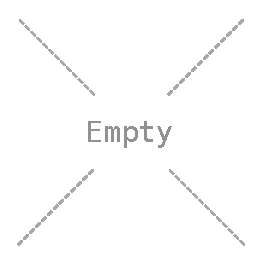
\includegraphics[height=\fgh]{empty.eps}

\mycaption{fig:usecase-battery}{Battery saver use case}{Energy-Security Tradeoff vs
   Strict Energy Budget as discussed in Section \ref{??}. 
The graph shows median sequential write total
   energy use with respect to time with respect to time.}


\end{figure}




% result
\figref{usecase-battery} shows the time versus
energy used. At 0 seconds, we begin writing. At 5 seconds, the ``battery
saver'' event occurs, causing the system to be underclocked. At 120
seconds, the system will die. If we blow past our energy ceiling, the
system will die.
The figure shows two lines:
%
{\bf (1)} {\em Freestyle Balanced only}, that
favors security even when backups are paused;  the device
dies before the I/Os complete.
%
{\bf (2)} {\em Freestyle Balanced $+$ ChaCha8}, that
performs the switch when the system enters the low power state. 
Our results show that, while the system uses slightly more power in the
short term, we stay within our energy budget and finish before the devices dies.
%
When we get the device to a charger (not shown), the cloud backup is enabled
again and when the nuggests are read, \sys automatically converges them back to 
Freestyle Balanced.

% overall result
On average, using forward switching resulted in a 3.3x total energy
reduction compared to exclusively using Freestyle Balanced, allowing us to
remain within our energy budget. \hsg{I don't see this 3.3x in the graph.
  Did you accidentally label the lines incorrectly?}.  We note, however,
that the energy savings is not the point of this experiment. Rather, the
lesson learned is that \sys enables the system to move to the right point
in the energy/security tradeoff space so that the current task can still
be accomplished before the battery is drained and without compromising
backup security at any point.


\hsg{we should exlude ChaCha8 only, unless you have a major point here}
\sout{{\bf (3)} {\em ChaCha8 only}
that favors low energy use even when backups are being uploaded;
the result shows that the device finish writing early but the file cannot
be uploaded to the cloud.}






% ===============================
\subsection{End-of-Life Device Slowdown} 
\label{subsec:uc3}


Another usecase of forward switchins is for offsetting the debilitating
decline in performance when storage devices such as SSDs reach end-of-life
(EoL); due to garbage collection and wear-leveling requirements of SSDs,
as free space becomes constrained, I/O performance drops
precipitously~\cite{SSDEOL1}.  Let us suppose in this case, the system
running on the dying SSDs have a strict latency budget (as long as meeting
some minimum security requirements).  The strict latency ceiling can be
violated if the device latency increases.  If \sys is made aware when the
drive is in such a state, we can offset some of the performance loss by
switching the ciphers of high traffic nuggets to the fastest acceptable
cipher available using forward switching.



\def \fgh {1in}

\begin{figure}[t] 

\centering

% {\input{data/usecase-eol-tradeoff.tex}} 

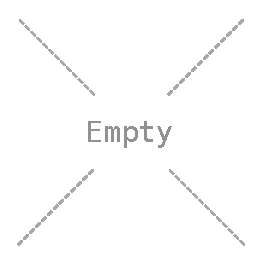
\includegraphics[height=\fgh]{empty.eps}

\mycaption{fig:usecase-eol-tradeoff}{Device end-of-life use case}{SSD EoL Use Case: 
Latency-Security Tradeoff vs Goals.  Median
   sequential and random 40MB read and write performance comparison: baseline
   versus simulated faulty block device.}

\end{figure}


To show this, we begin by writing 10 40MB files per each cipher as a
baseline. \hsg{I don't understand ``per each cipher''} We then introduce a
delay of $20ms$ simulating drive slowdown.
\hsg{Where do you get ``20ms'' from?  that's such a high latency. Any
  citation you can use here to back that up},
% --------------------------------------------------
\hsg{These sentences below are non informative. You should help reviewers
walk through the graph. I don't even understand what the x-axis in the Figure
means. The best way to describe a figure, is describe the x-axis and then y-axis,
and then pick two extreme points in the graph, and describe those points, what the
values mean, so that reviewers can really understand them. if reviewers understand
two extreme points, then they will undersstand the rest. Please redo the 
sentences.}
% --------------------------------------------------
\sout{
In \figref{usecase-eol-tradeoff}, we see the sequential and random read and
write performance of a 40MB workload when nuggets are encrypted exclusively with
our choice ciphers. While the latency ceiling and security floor have not
changed, we see increased latency in the delayed workloads.
Our goal is to remain under the latency ceiling while remaining above the
security floor. Thanks to Forward switching, accesses to highly trafficked areas
of the drive can remain performant even during drive end-of-life.}



% ================================================================
\subsection{Variable Security Regions} \label{subsec:uc2}

\hsg{here here here}

This usecase illustrates utility of spatial Selective switching to achieve a
performance win over prior work where the entire drive is encrypted with a
single cipher. We demonstrate \emph{Variable Security Regions} (VSR), where we
can choose to encrypt select files or portions of files with different keys and
ciphers below the filesystem level.

% background
Storing classified materials, corporate secrets, etc. require the highest level
of discretion, yet sensitive information like this can appear within a (much)
larger amount of data that we value less. But if only a small percentage of the
data needs the strongest encryption, then only a small percentage of the data
should have that associated overhead. In this scenario, a user wants to indicate
one or more regions of a file are more sensitive than the others. For example,
perhaps banking transaction information is littered throughout a PDF; perhaps
passwords and other sensitive information exists within several much larger
files. Using prior techniques, either all the data would be stored with high
overhead, the critical data would be stored without the mandated cipher type, or
the data would have to be split among separate files requiring potentially
complex and error-prone management schemes. SwitchCrypt VSRs allows us to
sidestep these issues.

% setup 
We begin by with 10 5MB and 4KB write-read operations to two
SwitchCrypt instances: one using ChaCha8 (C8) and the other using Freestyle
Strong (FreeStr). These results represent I/O without cipher switching where 100\% of
the data is stored with either high overhead (FS) or using an inappropriate
cipher (C8). We then use a third SwitchCrypt instance initialized with Selective
switching and write-read with a 7:3 ratio of ChaCha8 versus Freestyle
Balanced I/O operations. Here, 30\% of the data is considered sensitive. We
repeat this experiment three times.

\def \fgh {1in}

\begin{figure}[t]
    \centering
    %{\input{data/usecase-vsr-bar}}
    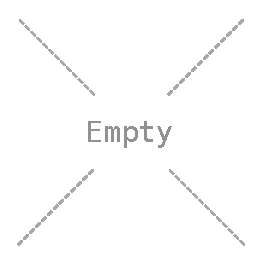
\includegraphics[height=\fgh]{empty.eps}
    \mycaption{fig:usecase-vsr-bar}{Selective file/region usecase}{VSR Use Case:
    ChaCha8 vs Freestyle Strong Sequential 4KB, 5MB Performance. The graph shows
    median sequential read and write performance comparison of 4KB, 5MB I/O with
    7-to-3 ratio, ChaCha8 vs Freestyle Strong (respectively).}
\end{figure}


% outcome
In \figref{usecase-vsr-bar}, we see the sequential read and write performance of
4KB and 5MB workloads when nuggets are encrypted exclusively with ChaCha8 or
Freestyle Balanced. Between them, we see Selective switching 7:3 ratio I/O
results.

Our goal is to use VSRs to keep our sensitive data at the mandated security
level while keeping the performance and battery life benefits of using a fast
cipher for the majority of I/O operations. Using SwitchCrypt Selective switching
versus prior work results in a reduction of 3.1x to 4.8x for read latency and
1.6x to 2.8x for write latency, all without compromising the security needs of
the most sensitive data.



% ===============================
\subsection{No-Downtime Encryption Upgrade} 
\label{subsec:uc3}




\def \fgh {1in}

\begin{figure}[t] 

\centering

% {\input{data/usecase-eol-tradeoff.tex}} 

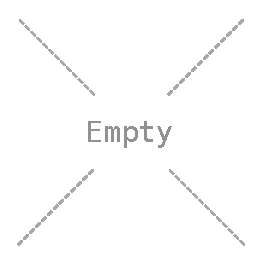
\includegraphics[height=\fgh]{empty.eps}

\mycaption{fig:usecase4}{No-downtime encryption upgrade}{.......}


\end{figure}


In \figref{usecase4} .........

\hsg{we must have a short case study here.
Otherwise no point of talking about mirrored switch}.

